冷气与暖气一样可以简化为一个以匀速在空间内上下移动的恒温热源,热源温度低于环境温度。当外界温度及室内初始物温度为35℃,室内温度设定为25度时,通过\eqref{final equation}可以得出随时间变化的房间温度分布。

房间内某几个时刻的温度分布如图\eqref{隔壁房间开冷气时的温度分布}所示。
\\
\begin{figure}[h]
    \centering
    \subfigure[空调刚开启时]{
    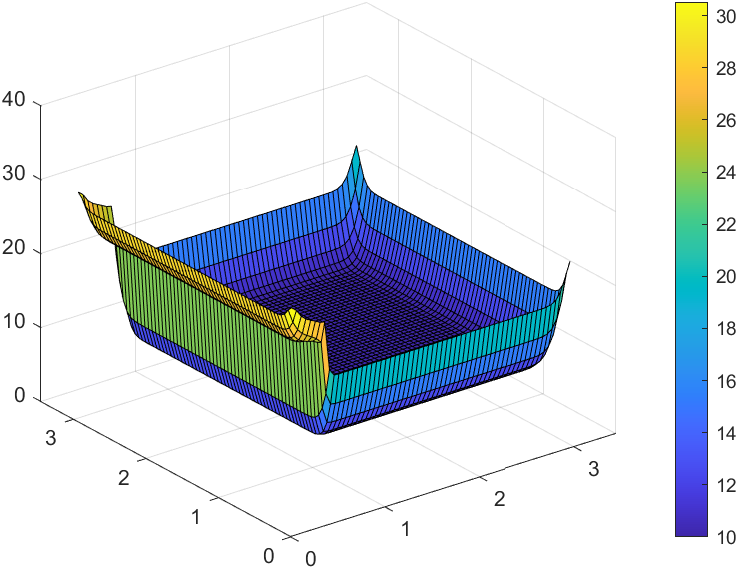
\includegraphics[width = 5.5cm]{figures/nr-cold-start.png}
    }\qquad
    \subfigure[空调向上扫风]{
    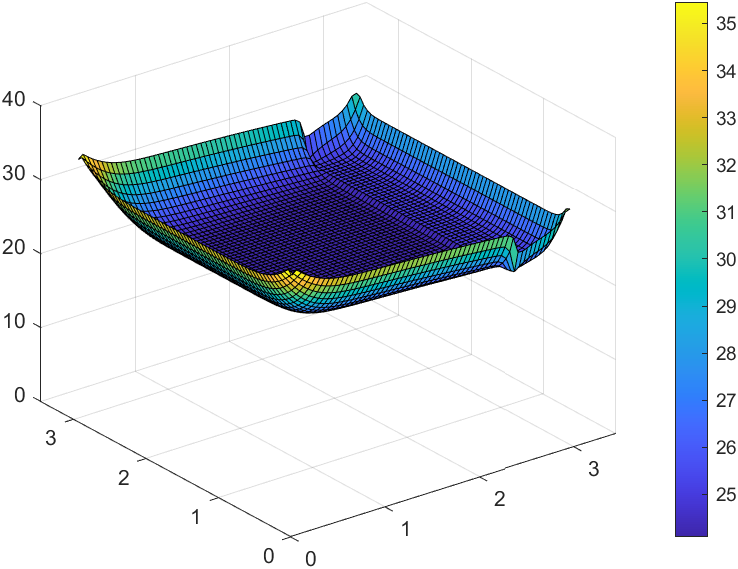
\includegraphics[width = 5.5cm]{figures/nr-cold-up.png}
    }\qquad
    \subfigure[空调向下扫风]{
    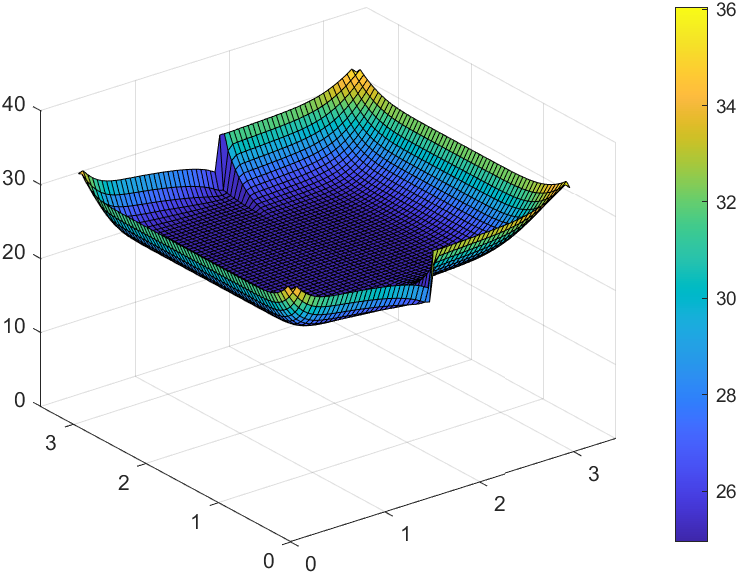
\includegraphics[width = 5.5cm]{figures/nr-cold-down.png}
    }\qquad
    \subfigure[房间竖直截面温度分布图]{
    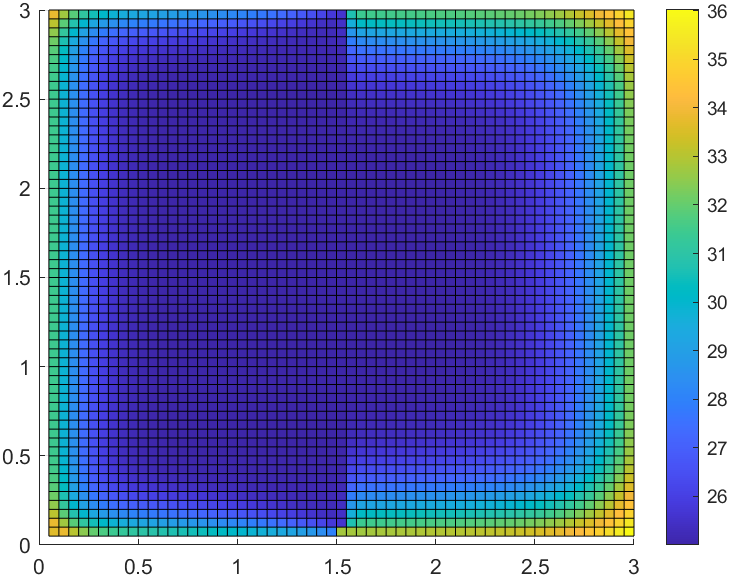
\includegraphics[width = 5.5cm]{figures/nr-cold-2d.png}
    }\qquad
    
    \caption{隔壁房间开冷气时的温度分布}
    \label{隔壁房间开冷气时的温度分布}
\end{figure}

可以得到设置25℃空调时,室内的平均温度为26.8℃,墙边的平均温度为31℃。因此在研究待测房间的传热过程时将31℃作为边界条件。
